% mnras_template.tex
%
% LaTeX template for creating an MNRAS paper
%
% v3.0 released 14 May 2015
% (version numbers match those of mnras.cls)
%
% Copyright (C) Royal Astronomical Society 2015
% Authors:
% Keith T. Smith (Royal Astronomical Society)

% Change log
%
% v3.0 May 2015
%    Renamed to match the new package name
%    Version number matches mnras.cls
%    A few minor tweaks to wording
% v1.0 September 2013
%    Beta testing only - never publicly released
%    First version: a simple (ish) template for creating an MNRAS paper

%%%%%%%%%%%%%%%%%%%%%%%%%%%%%%%%%%%%%%%%%%%%%%%%%%
% Basic setup. Most papers should leave these options alone.
\documentclass[a4paper,fleqn,usenatbib]{mnras}

% MNRAS is set in Times font. If you don't have this installed (most LaTeX
% installations will be fine) or prefer the old Computer Modern fonts, comment
% out the following line
\usepackage{newtxtext,newtxmath}
% Depending on your LaTeX fonts installation, you might get better results with one of these:
%\usepackage{mathptmx}
%\usepackage{txfonts}

% Use vector fonts, so it zooms properly in on-screen viewing software
% Don't change these lines unless you know what you are doing
\usepackage[T1]{fontenc}
\usepackage{ae,aecompl}


%%%%% AUTHORS - PLACE YOUR OWN PACKAGES HERE %%%%%

% Only include extra packages if you really need them. Common packages are:
\usepackage{graphicx}	% Including figure files
\usepackage{amsmath}	% Advanced maths commands
\usepackage{amssymb}	% Extra maths symbols

%%%%%%%%%%%%%%%%%%%%%%%%%%%%%%%%%%%%%%%%%%%%%%%%%%

%%%%% AUTHORS - PLACE YOUR OWN COMMANDS HERE %%%%%

% Please keep new commands to a minimum, and use \newcommand not \def to avoid
% overwriting existing commands. Example:
%\newcommand{\pcm}{\,cm$^{-2}$}	% per cm-squared

%%%%%%%%%%%%%%%%%%%%%%%%%%%%%%%%%%%%%%%%%%%%%%%%%%

%%%%%%%%%%%%%%%%%%% TITLE PAGE %%%%%%%%%%%%%%%%%%%

% Title of the paper, and the short title which is used in the headers.
% Keep the title short and informative.
\title[Galactic Thermal Evaporation]{Galactic thermal evaporation and the implications for low-mass haloes.}

% The list of authors, and the short list which is used in the headers.
% If you need two or more lines of authors, add an extra line using \newauthor
\author[Selsing]{
Jonatan Selsing,$^{1}$\thanks{E-mail: jselsing@dark-cosmology.dk}
\\
% List of institutions
$^{1}$Dark Cosmology Centre, Niels Bohr Institute, University of Copenhagen, Juliane
Maries Vej 30, 2100 Copenhagen, Denmark.}

% These dates will be filled out by the publisher
\date{Accepted XXX. Received YYY; in original form ZZZ}

% Enter the current year, for the copyright statements etc.
\pubyear{2015}






% TO DOS
\newcommand{\todo}[3]{{\color{#2}\emph{#1}: #3}}
\newcommand{\changed}[1]{\todo{}{green}{#1}}
\newcommand{\jtodo}[1]{\todo{TODO }{red}{#1}}
\newcommand{\qtodo}[1]{\todo{Question}{red}{#1}}







% Don't change these lines
\begin{document}
\label{firstpage}
\pagerange{\pageref{firstpage}--\pageref{lastpage}}
\maketitle

% Abstract of the paper
\begin{abstract}
A gas of ions sitting in a galaxy, if we assume that it is collisionally ionised, will have some characteristic temperature relevant to that species depending on the ionisation potential of the species. At this characteristic temperature the velocity distribution of gas molecules will follow the Maxwell-Boltzmann distribution. For a given halo with some mass there will be some espace velocity. Some fraction of the gas, due to the distribution of velocities, will have a velocity which exceeds the escape velocity of the halo and will therefore escape. In the gas itself the mean-free-path of the particles will be short compared to the length-scales which the gas need to escape due to the assumption of collisional excitation, but at the interface between the gas and the IGM, som fraction of the gas will be able to escape. This should lead to a net escape of atoms from the halo and behave similar to evaporation. This additionally requires that the cooling timescale for the ion is longer than the characteristic timescale for escape. 

This process is very similar to the process which describes evaporation from a water-surface, where some small fraction of the water-molecules at the interface between the water and air will have a finite chance of moving out of the water. Or somewhat equivalently the escape of the lighter elements from the atmospheres of planets. 
%This is a simple template for authors to write new MNRAS papers.
%The abstract should briefly describe the aims, methods, and main results of the paper.
%It should be a single paragraph not more than 250 words (200 words for Letters).
%No references should appear in the abstract. This is the coolest thing you will read, ever!
\end{abstract}

% Select between one and six entries from the list of approved keywords.
% Don't make up new ones.
\begin{keywords}
keyword1 -- keyword2 -- keyword3
\end{keywords}

%%%%%%%%%%%%%%%%%%%%%%%%%%%%%%%%%%%%%%%%%%%%%%%%%%

%%%%%%%%%%%%%%%%% BODY OF PAPER %%%%%%%%%%%%%%%%%%

\section{Introduction}

Gas dynamics on galactic scales are controlled by the thermal pressure of the gas and the radiation pressure of the stars equilibrated to the compressional pressure of gravity. Radiative cooling, either though continuum emission or line-emission allows the gas to contract under gravity whereas feedback processes such as stellar winds, supernovae and AGNs causes the gas to expand. 

Ionic species in varying degrees of ionization is observed in galaxies and assuming that they are collisionally exited, indicates that for each ionic species considered, different effective local temperatures regulate the thermal pressure of the gas. Since the effective temperature is a generalization of the average kinetic energy of the gas, this corresponds to a distribution of particle velocities given by the Maxwell-Boltzmann distribution. At any given time for a gas in thermal equilibrium, there will be particles with high velocity and particles with low velocity. Due to the assumption of thermal equilibrium, the gas particles will not travel far before another particle is encountered and the kinetic energy shared. At the edge of a cloud, however, there will be a chance for the gas to escape given that the mean-free-path of the particle is longer than the interface between the gas and the surrounding material. In the universe, gas is confined by it's own self-gravity, but for a given gravitational potential generated by the gas and the nascent dark-matter halo, there will be an escape velocity which will allow a gas particle to escape. This is very similar to thermal evaporation of water, as we know from Earth, where the velcity can overcome the " chemical potential " of the water and turn to vapor. Given enough time, all gas in galaxies should in principle escape, but the time-scale for this is extremely long, however for high-ionization gasses which have a high effective collisional equilibration temperature sitting in low-mass haloes, potentially some fraction of the gas will escape on at time-scale shorter than a few dynamical time-scales. 
In this letter we try to calculate the mass-loss rate for a given ionic species and assess the implication for low-mass haloes, especially explaining the missing \ion{CIV} in very low-mass haloes found by Burchett et al.  

\jtodo{Limitations: One issue would be if the high-ionization gas is embedded in a cooler gas making the mean-free-path short compared to the escape scale.} 


\jtodo{A discussion of hydrodynamical escape versus thermal escape.}

%This is a simple template for authors to write new MNRAS papers.
%See \texttt{mnras\_sample.tex} for a more complex example, and \texttt{mnras\_guide.tex}
%for a full user guide.
%
%All papers should start with an Introduction section, which sets the work
%in context, cites relevant earlier studies in the field by ,
%and describes the problem the authors aim to solve \citep[e.g.][]{Bromberg2011b}.

\section{Methods, Observations, Simulations etc.}
\label{sec:Methods} % used for referring to this section from elsewhere
%Normally the next section describes the techniques the authors used.
%It is frequently split into subsections, such as Section~\ref{sec:maths} below.
In this work, two approaches to the calculation of the mass-loss rate of gas due to thermal evaporation are attempted. The upper limit is provided by the classical Jeans escape \citep{Jeans1925} in which a high-velocity tail of the Maxwell-Boltzmann velocity distribrution is assumed to be populated at all times and the continuity equation is used to find the mass-loss rate. The lower limit on the escape-rate is provided by the 'lid'-approximation \citep{Gross1974} in which the high-velocity end of the velocity distribution is assumed re-populated on some timescale after which a 'lid' is lifted and the high-velocity end is allowed to escape. 
Common for both methods are the exploitation of the Maxwell-Boltzmann distribution which is the probability for a single particle in a thermally equilibrated gas to have a certain velocity based on internal energy of the gas, 

\begin{equation}
f(v)=\sqrt{ \left( \frac{m}{2 \pi k T}  \right)^3 } 4 \pi v^2 e^{-\frac{mv^2}{2 k T}},
\label{eq:Boltzmann}
\end{equation}

where $v$ is the velocity, $m$ is the particle mass, $k$ is the Boltzmann constant and $T$ is the gas temperature.

Another quantity of prime importance to this calculated is the escape velocity of a particle in a gravitational potential which is the velocity with which a particle has enough energy to escape to infinity from a isolated potential. The escape velocity is given by 

\begin{equation}
v_{esc} = \sqrt{ \frac{2 G M(<r)}{r}},
\label{eq:escape}
\end{equation}
where $r$ is the radius and $m(<r)$ is the mass contained with the radius, $r$. Assuming an NFW-profile \citep{Navarro1995} for the halo in which the gas is embedded, allows us to calculate the escape velocity as a function of radius for a halo of any given mass. \jtodo{Think more about what escape velocity to use - use the maximum over the entire profile or max of outer escape-layer}


\subsection{Jeans escape}
\label{sec:Jeans} 

The flux of escaping particles is found by integrating the Maxwell-Boltzmann distribution from the escape velocity and up in three dimensions and multiplying with the number density of particles

\begin{equation}
v_{esc} = \sqrt{ \frac{2 G M(<r)}{r}},
\label{eq:Jeansflux}
\end{equation}


% used for referring to this section from elsewhere
%Simple mathematics can be inserted into the flow of the text e.g. $2\times3=6$
%or $v=220$\,km\,s$^{-1}$, but more complicated expressions should be entered
%as a numbered equation:





Refer back to them as e.g. equation~(\ref{eq:quadratic}).

\subsection{Figures and tables}

Figures and tables should be placed at logical positions in the text. Don't
worry about the exact layout, which will be handled by the publishers.

Figures are referred to as e.g. Fig.~\ref{fig:example_figure}, and tables as
e.g. Table~\ref{tab:example_table}.


\begin{figure}
	% To include a figure from a file named example.*
	% Allowable file formats are eps or ps if compiling using latex
	% or pdf, png, jpg if compiling using pdflatex
	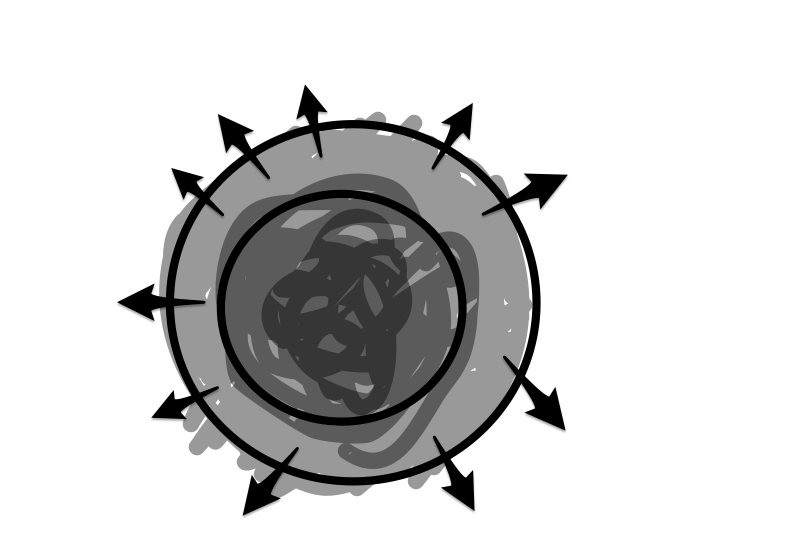
\includegraphics[width=\columnwidth]{figures/Thermal_escape.png}
    \caption{Schematic illustration of the thermal evaporation. \jtodo{Placeholder}}
    \label{fig:example_figure}
\end{figure}

% Example table
\begin{table}
	\centering
	\caption{This is an example table. Captions appear above each table.
	Remember to define the quantities, symbols and units used.}
	\label{tab:example_table}
	\begin{tabular}{lccr} % four columns, alignment for each
		\hline
		A & B & C & D\\
		\hline
		1 & 2 & 3 & 4\\
		2 & 4 & 6 & 8\\
		3 & 5 & 7 & 9\\
		\hline
	\end{tabular}
\end{table}


\section{Conclusions}

The last numbered section should briefly summarise what has been done, and describe
the final conclusions which the authors draw from their work.

\section*{Acknowledgements}

The Acknowledgements section is not numbered. Here you can thank helpful
colleagues, acknowledge funding agencies, telescopes and facilities used etc.
Try to keep it short.

%%%%%%%%%%%%%%%%%%%%%%%%%%%%%%%%%%%%%%%%%%%%%%%%%%

%%%%%%%%%%%%%%%%%%%% REFERENCES %%%%%%%%%%%%%%%%%%

% The best way to enter references is to use BibTeX:

\bibliographystyle{mnras}
\bibliography{references} % if your bibtex file is called example.bib


% Alternatively you could enter them by hand, like this:
% This method is tedious and prone to error if you have lots of references
%\begin{thebibliography}{99}
%\bibitem[\protect\citeauthoryear{Author}{2012}]{Author2012}
%Author A.~N., 2013, Journal of Improbable Astronomy, 1, 1
%\bibitem[\protect\citeauthoryear{Others}{2013}]{Others2013}
%Others S., 2012, Journal of Interesting Stuff, 17, 198
%\end{thebibliography}

%%%%%%%%%%%%%%%%%%%%%%%%%%%%%%%%%%%%%%%%%%%%%%%%%%

%%%%%%%%%%%%%%%%% APPENDICES %%%%%%%%%%%%%%%%%%%%%

\appendix


%%%%%%%%%%%%%%%%%%%%%%%%%%%%%%%%%%%%%%%%%%%%%%%%%%


% Don't change these lines
\bsp	% typesetting comment
\label{lastpage}
\end{document}

% End of mnras_template.tex